\documentclass[10pt,twocolumn]{article}
\usepackage[letterpaper,margin=0.72in,columnsep=0.25in]{geometry}
\usepackage{booktabs,graphicx,amsmath,amssymb,tabularx,array,xcolor,hyperref,xspace}
\hypersetup{hidelinks,pdftitle={Agora: One Sentence, One Living World}}
\newcommand{\agora}{\textsc{Agora}\xspace}
\newcommand{\systemvision}{\emph{One Sentence, One Living World}}
\title{\textbf{Agora: One Sentence, One Living World}\\
Generating High-Quality Worlds for Human--AI Social Interaction}
\author{Boxun Xu \and Yueze Wang \and Peng Li}
\date{}

\begin{document}
\maketitle

\begin{abstract}
Can one sentence produce a world that is visually and structurally coherent,
and also rich enough for humans, AI agents, and other players to act together?
We present \agora, a language-to-world system organized around three connected
goals: one-sentence authoring, coherent playable worlds, and consequential
interaction among humans and AI agents. A structured world representation
grounds agents in rooms, roles, inventories, institutions, and evolving
relationships. Each world offers recognizable actions while also allowing an
actor to propose context-specific speech, exchange, creation, or status change;
a World Coordinator evaluates feasibility, consent, and resource constraints
before shared state changes. We evaluate five worlds generated from five
one-sentence premises. On ten paired premises, compositional generation yields
complete worlds in 10/10 cases versus 7/10 for a strong single-pass generator;
five worlds also satisfy visual coherence, persistence, and interactive-use
criteria. Matched two-round language-model runs across those worlds produce 53
events: 37 unique dyads, 13 AI-to-human interactions, nine premise-specific
actions, and ten approved open proposals. The action-result
success rate is 87.5\%.
We first report a descriptive analysis of three previously completed 100-agent
runs comprising 1,052 events. The worlds contain 229--282 unique
interaction dyads, with 23.4--36.5\% of events returning to an existing dyad.
Their social trajectories differ with the
world premise: a black-market world accumulates influence/fear change, whereas
a storm-struck cruise and an adventuring guild accumulate predominantly trust
and affection. These observations reveal persistent, world-conditioned social
processes and motivate a paired intervention: seed a flood threat as private
knowledge in a 25-agent tidal embassy, then compare complete social memory with
a memory ablation across matched random seeds. Primary outcomes measure
information diffusion and coordinated response; secondary outcomes measure
network formation, spatial transmission, object use, and norm violations.
This connects language-to-world generation with an experimental science of what
happens inside generated worlds.
\end{abstract}

\section{Introduction}

In the Smallville study, a single initial intention---one resident planning a
Valentine's Day party---spread through a town and produced invitations,
coordination, and attendance \cite{park2023}. Local memories and encounters
developed into a community-level process, making the town itself part of the
experimental phenomenon.

Systems that generate interactive worlds from language face a complementary
challenge: the world must support a society as well as a scene. Place,
property, institutions, accumulated relationships, and material consequences
must shape what inhabitants perceive and do.

We study generated worlds as \emph{experimental environments}. Given a premise,
\agora generates explicit rooms, roles, items, rules, knowledge policies, agent
profiles, and visual identity as a persistent shared world. Agents perceive a
bounded local context, select situated actions, move, trade, create objects,
and update memories and directed relationships. The research object is the
resulting trajectory
\[
  \tau = (S_0, a_1, S_1, \ldots, a_T, S_T),
\]
where each state records social, spatial, and material consequences.

This paper makes four contributions. First, it connects one-sentence authoring
to coherent visual, spatial, social, and material world generation. Second, it
offers world-specific actions through one interface shared by
humans and AI agents while allowing coordinator-governed novel actions. Third, it
introduces a trajectory-based evaluation suite
for diffusion, coordination, network formation, spatial behavior, relationships,
objects, and norms. Fourth, it reports a controlled five-world interaction study,
a descriptive analysis of three longer real runs, and
preregisters a paired causal experiment in which the same agents face the same
event with or without persistent social memory.

\begin{figure*}[t]
\centering
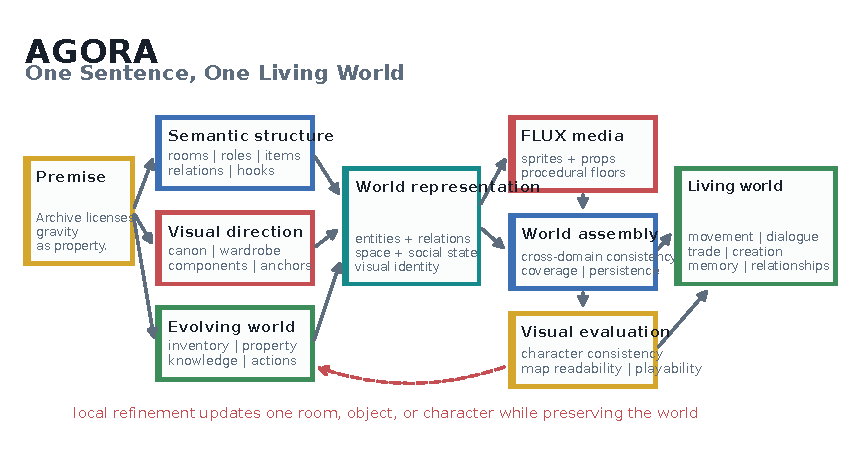
\includegraphics[width=0.97\textwidth]{figures/generation_overview.pdf}
\caption{The central research progression of \agora. A sentence expands into
semantic, visual, spatial, and social structure; complementary evaluations
establish coherence and playability. Humans and agents then act through both
world-specific actions and open proposals, producing trajectories that can
be studied as social processes.}
\label{fig:generation-overview}
\end{figure*}

\section{Research Thesis and Questions}

Our thesis is \systemvision. The phrase has three independently falsifiable
parts. \textbf{One sentence} is an authoring claim: the premise supplies world
semantics while the generation method supplies a reusable structure.
\textbf{One living world} is a world-quality claim: the output forms a coherent,
persistent, playable environment. \textbf{Living} is an interaction claim:
humans and agents must be
able to form intentions that change shared social, spatial, and material state.

This decomposition yields four research questions:
\begin{description}
  \item[RQ1: World construction.] Can compositional generation turn diverse
  one-sentence premises into complete, visually grounded, interactive worlds
  more reliably than a matched single-pass generator?
  \item[RQ2: Interaction breadth.] Does each world expose multiple meaningful
  action families to both human and AI actors, with consequences in shared
  world state?
  \item[RQ3: Intentional openness.] Can an actor express a context-specific
  intention outside the generated repertoire while a coordinator preserves
  legality, consent, and bounded effects?
  \item[RQ4: Social process.] Do fresh and historical interactions show repeated
  ties, world-conditioned action choices, and persistent relational change that
  motivate a controlled long-horizon community experiment?
\end{description}

The evaluation follows these questions in sequence. Paired generation studies
address RQ1; action coverage and interactive trials address RQ2;
coordinator decisions and enacted proposals address RQ3; and interaction
trajectories address RQ4.

\section{Related Work}

\paragraph{Persistent agent communities.}
Generative Agents introduced observation, memory retrieval, reflection, and
planning in a spatial town populated by 25 agents \cite{park2023}. Its
ablation and human evaluation connect architectural components to believable
individual and emergent behavior. \agora shares the interest in persistent
communities but varies the world itself: institutions, resources, available
actions, and geometry are generated from language for each premise.

\paragraph{Social evaluation.}
SOTOPIA evaluates goal-directed social interaction across cooperation,
competition, exchange, and negotiation \cite{zhou2024}. It connects language
behavior to social goals and partner judgments. Our analysis extends across
multi-round population processes grounded in persistent world state. Concordia similarly frames LLM simulations as
generative agent-based models whose actions are grounded in physical, social,
or digital space \cite{vezhnevets2023}; \agora adds language-authored interactive
worlds and multimodal, object-level state.

Recent social simulators expand population scale and experimental scope.
AgentSociety combines LLM-driven agents with a realistic environment and uses
interventions to study diffusion, policy, and external shocks
\cite{agentsociety}. LMAgent demonstrates multimodal behavior at large scale in
an e-commerce society \cite{lmagent}, while Avalon-based work analyzes
collaboration and confrontation under fixed game rules \cite{avalon}. These
systems strengthen the case for population-level analysis. \agora asks an
upstream question: can the experimental environment itself be generated from a
sentence while retaining stateful, inspectable social action?

\paragraph{Generated interactive environments.}
Language-to-game and procedural-generation systems typically emphasize content
validity, controllability, and playability. We connect these properties to a
second object of study: whether generated institutions and action possibilities
alter collective behavior.

Word2World, DreamGarden, and related language-to-game systems broaden the scope
of prompt-based authoring \cite{word2world,dreamgarden}. Learned interactive
world models such as Genie emphasize controllable visual experience
\cite{genie}. Voyager studies open-ended embodied skill acquisition in a fixed
Minecraft environment and shows the value of feedback and self-verification
\cite{voyager}. \agora varies the world definition itself, generates explicit
ownership and institutions, and then asks what social processes each resulting
environment permits.

\begin{table}[t]
\centering
\small
\setlength{\tabcolsep}{2pt}
\begin{tabularx}{\columnwidth}{l*{4}{>{\centering\arraybackslash}X}}
\toprule
System & Gen. world & Persistent society & Open action & Human co-play \\
\midrule
Smallville \cite{park2023} & -- & \checkmark & language & observer \\
SOTOPIA \cite{zhou2024} & -- & -- & dialogue & dyadic \\
Concordia \cite{vezhnevets2023} & authored & \checkmark & GM & researcher \\
Voyager \cite{voyager} & -- & memory & code skills & instr. \\
\agora & \checkmark & \checkmark & coord. & shared world \\
\bottomrule
\end{tabularx}
\caption{Conceptual comparison. ``Gen. world'' means the interactive social and
material substrate is generated from the premise together with its inhabitants.}
\label{tab:related}
\end{table}

The closest conceptual analogue to our World Coordinator is Concordia's Game
Master: agents describe intended actions in language and a separate component
grounds them in the environment. In \agora, each world's rules shape the
coordinator's decisions, and accepted actions update inventory, relationships,
objects, and status. The coordinator thereby connects interpretation with an
observable change in shared world state.

\section{From a Sentence to a High-Quality World}

\subsection{World Representation and Quality Criteria}

Given premise $p$, \agora constructs
\[
W=(E,G,R,K,A,M,P),
\]
where $E$ contains rooms, agents, items, and institutions; $G$ is traversable
geometry; $R$ contains physical, economic, and social rules; $K$ allocates
public and private knowledge; $A$ is the available action space; $M$ associates
visual media with world entities; and $P$ records stable world identity. The
evolving state $S_t$ describes the world at time $t$.

We evaluate four complementary properties. Semantic completeness requires each
entity and relation to be well defined. Cross-modal coherence requires maps,
rooms, characters, and objects to share the intended identity and visual
language. Spatial quality requires navigable geometry and readable placement.
Interactive persistence requires movement, messaging, object use, trade, and
their consequences to remain observable across continued play. The final
interactive evaluation included 25 rendered agents and a model-mediated reply.

\subsection{Compositional Generation and Local Refinement}

A planning stage establishes institutions, conflicts, resources, and activity
loops. Specialized stages then develop materials, rooms, items, roles, main
characters, knowledge, visual style, wardrobe, property, and placement. Their
dependencies make local refinement possible: an empty inventory revisits the
character--item relation, an unreadable object revisits visual placement, and
an inconsistent character revisits character generation while the rest of the
world remains stable.

In the paired generation study, ten premises use the same Gemini model and
temperature for the compositional method and a strong single-pass baseline.
The baseline receives a 24,576-token output allowance, three times the maximum
of any specialized stage. Compositional generation produces complete worlds in
10/10 cases versus 7/10 for the baseline; first-pass completion is 9/10 versus
5/10. The single-pass method uses approximately half as many tokens and is
1.8--1.9$\times$ faster, revealing a reliability--cost tradeoff.

For five seeded role inconsistencies, localized refinement restores all five
worlds while preserving five unaffected intermediate stages, reducing model
calls by 48.0\% and tokens by 39.9\% relative to complete regeneration. The
multimodal evaluation identifies all 58 injected defects with no false
positives. These results establish the world-quality basis for the subsequent
social study.

\begin{figure*}[t]
\centering
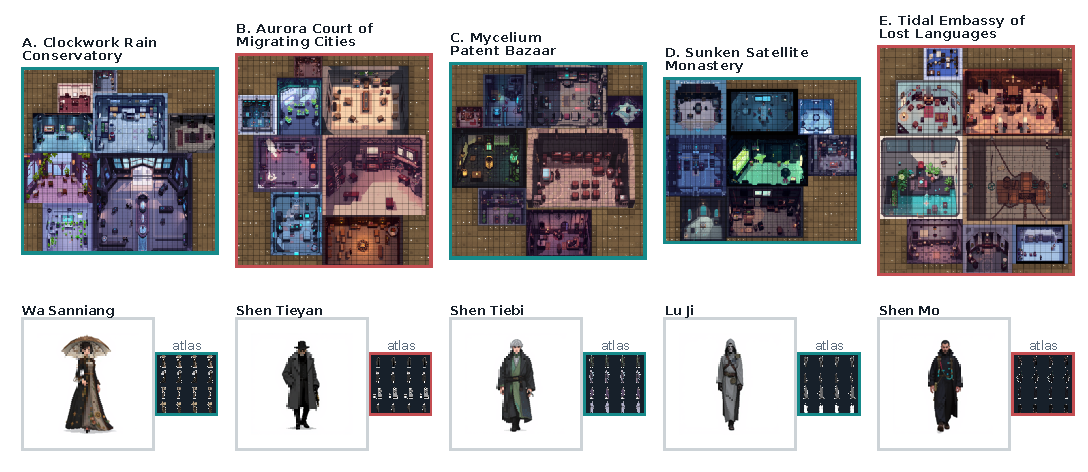
\includegraphics[width=0.96\textwidth]{figures/generated_worlds.pdf}
\caption{Five complete worlds generated by the same one-sentence method:
Clockwork Rain Conservatory, Aurora Court of Migrating Cities, Mycelium Patent
Bazaar, Tidal Embassy of Lost Languages, and Sunken Satellite Monastery. The
interaction study follows inhabitants acting inside these worlds.}
\label{fig:worlds}
\end{figure*}

\begin{table}[t]
\centering
\small
\begin{tabularx}{\columnwidth}{X>{\centering\arraybackslash}p{0.23\columnwidth}>{\centering\arraybackslash}p{0.19\columnwidth}}
\toprule
Quality evidence & Compositional & Single-pass \\
\midrule
Complete world & 10/10 & 7/10 \\
First-pass complete & 9/10 & 5/10 \\
Localized role refinement & 5/5 & -- \\
Injected defects detected & 58/58 & -- \\
False positives & 0/58 & -- \\
Visually grounded playable worlds & 5 & -- \\
\bottomrule
\end{tabularx}
\caption{World-generation evidence preceding the interaction study. The rows
measure complementary aspects of completeness, visual quality, and refinement.}
\label{tab:quality}
\end{table}

\begin{figure*}[t]
\centering
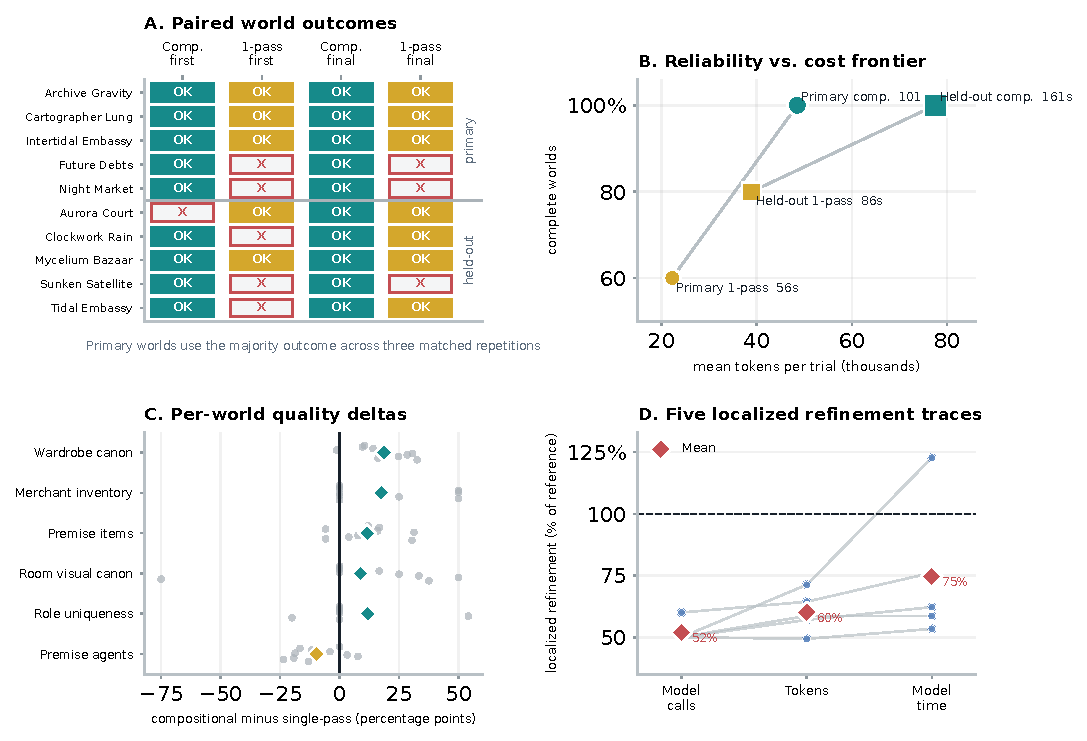
\includegraphics[width=0.92\textwidth]{figures/world_quality_results.pdf}
\caption{World-quality evidence preceding the social study. (A) Paired
first-pass and final outcomes on ten premises. (B) Completion, token use, and
latency reveal a reliability--cost tradeoff. (C) Per-world differences locate
where compositional generation helps. (D) Local refinement reduces calls and
tokens while preserving unaffected world structure.}
\label{fig:quality-results}
\end{figure*}

Figure~\ref{fig:quality-results} separates reliability, semantic coverage,
visual coherence, latency, and refinement locality. The single-pass generator
is faster and cheaper, while the compositional method completes more worlds.
These differences matter for the interaction study because ownership,
character identity, room geometry, and object availability determine who can
meet, what can be transferred, and which social consequences become observable.

\subsection{A Generated World in Detail: Tidal Embassy}

We now follow \emph{Tidal Embassy of Lost Languages} from premise to play. Its
one-sentence premise describes a
floating embassy where linguists, smugglers, ambassadors, and memory divers
trade endangered languages as political assets. The example preserves
intermediate images and refinement attempts, allowing each generative stage to
be connected to the final playable world.

\paragraph{Step 1: Premise analysis and planning.}
The planning stage identifies the nouns that become state---embassy,
languages, translation rights, archives, smugglers, diplomats, and tides---and
the verbs that imply gameplay---trade, translate, forge, authenticate, rescue,
and reveal. It then proposes an institutional loop: access to archives produces
linguistic objects; translators and forgers can
translate or forge them; diplomats exchange rights and debts; customs officers
can inspect transfers; flood events threaten stored knowledge. The resulting
world plan connects entities, conflicts, resource cycles, and open questions.

Planning establishes what must exist and why it matters. Later stages determine
spatial layout, visual appearance, and resource quantities. Missing activity
loops are refined before visual generation; for example, translation rights
must have a source, a use, and a means of transfer.

\paragraph{Step 2: Semantic structure.}
Semantic generation expands the plan into rooms, roles, items, institutions,
knowledge, and conflict hooks with stable identities. In this world,
the graph contains eight rooms, including the Phoneme Exchange, Mnemonic
Garden, Embassy Customs and Quarantine, and Ballast Hold; 25 named main
characters; and 20 distinct items. Explicit relations connect each character to
a home, each possession to an owner, and each action to relevant role,
knowledge, location, or resource conditions.

The generation process also preserves asymmetry. Shen Mo is a Phonetic
Smuggler and Lexical Restorationist based in the Cartographer's Nook. His
inventory includes a translation ear-cuff, archive key, forged exchange ledger,
dive helmet, ritual ink, and a fragment of the Unspoken Treaty. His private
knowledge includes phonetic decay patterns and ventilation shafts linking
Customs to the Mnemonic Garden. Another character receives different property,
authority, and information. This uneven allocation is what later makes
persuasion, trade, secrecy, and coalition formation possible.

\paragraph{Step 3: Visual direction and cross-modal identity.}
The visual direction converts semantic identity into a shared canon:
Art Nouveau diplomatic architecture, floating platforms, brass infrastructure,
bioluminescent language media, water intrusion, and a melancholic ritual tone.
It also emits per-entity appearance anchors. Room prompts inherit the canon but
add function-specific materials; character prompts inherit world palette and
wardrobe rules but retain role silhouettes; props receive icons whose shapes
communicate their use. Shared style and entity-specific appearance jointly keep
rooms, inhabitants, and objects recognizable as parts of the same world.

The visual direction guides each image independently while maintaining common
architecture, materials, palette, and role silhouettes. A visual inconsistency
can therefore be refined locally while the semantic identity of the world
remains stable.

\begin{figure*}[t]
\centering
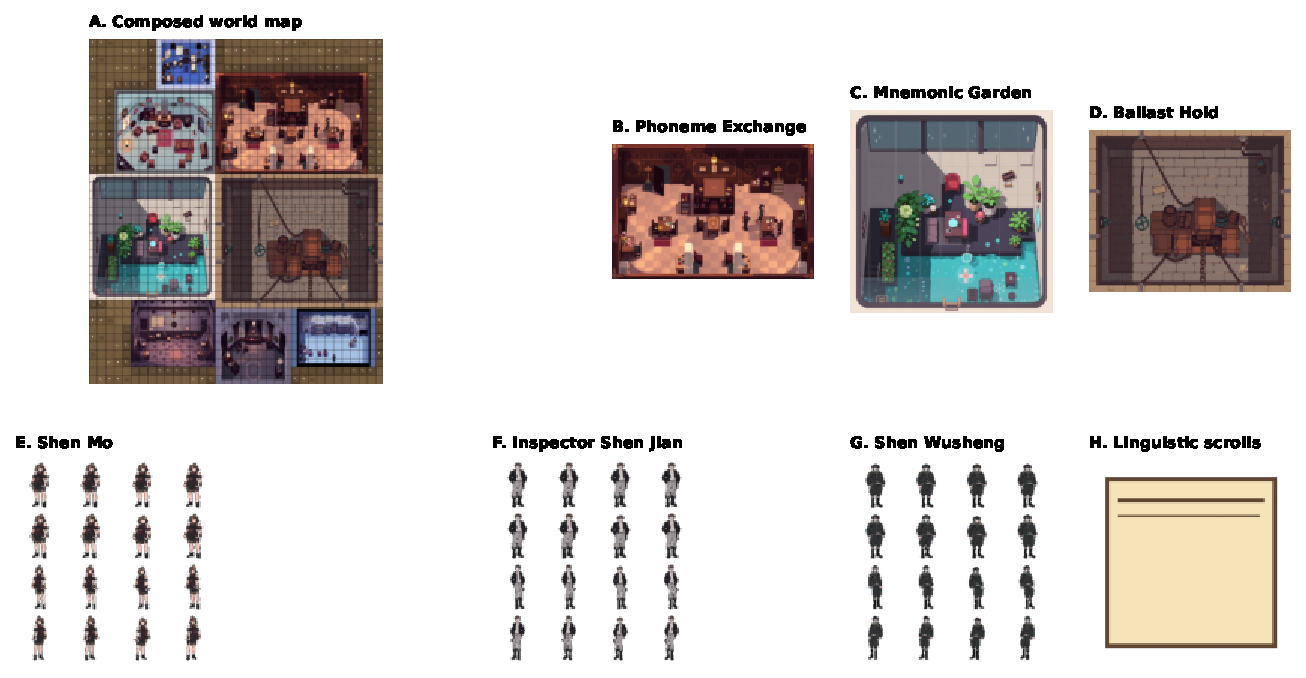
\includegraphics[width=0.98\textwidth]{figures/tidal_embassy_visual_elements.pdf}
\caption{Generated visual elements from Tidal Embassy. The composed map contains
eight generated floors (A--D show the map and three constituent rooms); E--G
show the latest directional character atlases; H is a generated object. Shared
visual motifs connect spatial, character, and object identity.}
\label{fig:tidal-visual-elements}
\end{figure*}

\paragraph{Step 4: Evolving world state.}
This stage determines what can change after the images are produced.
It creates wallets, inventories, property libraries, knowledge assets, directed
relationships, task threads, room occupancy, and world-event status. It also
defines invariants. Item quantities remain nonnegative; physical transfers
conserve quantity; private knowledge has an owner and an acquisition event; a
character occupies one reachable coordinate; relationship changes are directed.
Tidal's initial action repertoire contains seven general actions, one event-scale
action, and nine forms of open action, all linked to the same world state.

The evolving state connects generated descriptions through observable causes
and consequences. The treaty fragment in Shen Mo's inventory can later be inspected,
given away, stolen through an allowed rule, or used as an input to another
action. When ownership changes, the next observation shows the new owner.

\paragraph{Step 5: Integrated world representation.}
The integrated representation connects semantic, visual, spatial, and evolving
state. It supports cross-domain questions:
Does every home room exist? Does every main character have a visual asset and a
walkable placement? Is an item used by an action defined and obtainable? Does a
private fact mention an existing institution? Does a room's purpose agree with
its objects and activities? These dependencies guide local refinement.

If a character image is inconsistent, roles, rooms, and items remain fixed. If
an item relation is missing, only the connected content is regenerated. Figure
\ref{fig:tidal-repair} illustrates this process: two room images are refined
while the rest of Tidal Embassy remains unchanged.

\paragraph{Step 6: Visual generation.}
FLUX generates the map source, individual room floors, characters, and local
objects from the shared visual direction. Character images are arranged into
directional movement atlases, and room images are placed within the planned
regions and connected by traversable corridors. Figure
\ref{fig:tidal-visual-elements} shows the composed map alongside three source floors,
three latest character atlases, and an object.

Functional visibility connects visual quality to use: room imagery must cover
its playable area, characters must remain recognizable while moving, and
furniture must preserve navigable paths.

\paragraph{Step 7: Visual and spatial evaluation.}
The evaluation examines semantic completeness, visual identity, traversable
geometry, foreground coverage, directional character consistency, readable
room composition, and visibility during play. The Diplomat's Lounge required
three real generation attempts. Attempt 1 was classified as a poster card with
an edge blank-background ratio of 0.56. Attempt 2 removed the card appearance
but retained a blank-margin failure with a maximum blank-row ratio of 0.73.
Only the third, edge-to-edge playable floor was accepted.

\begin{figure*}[t]
\centering
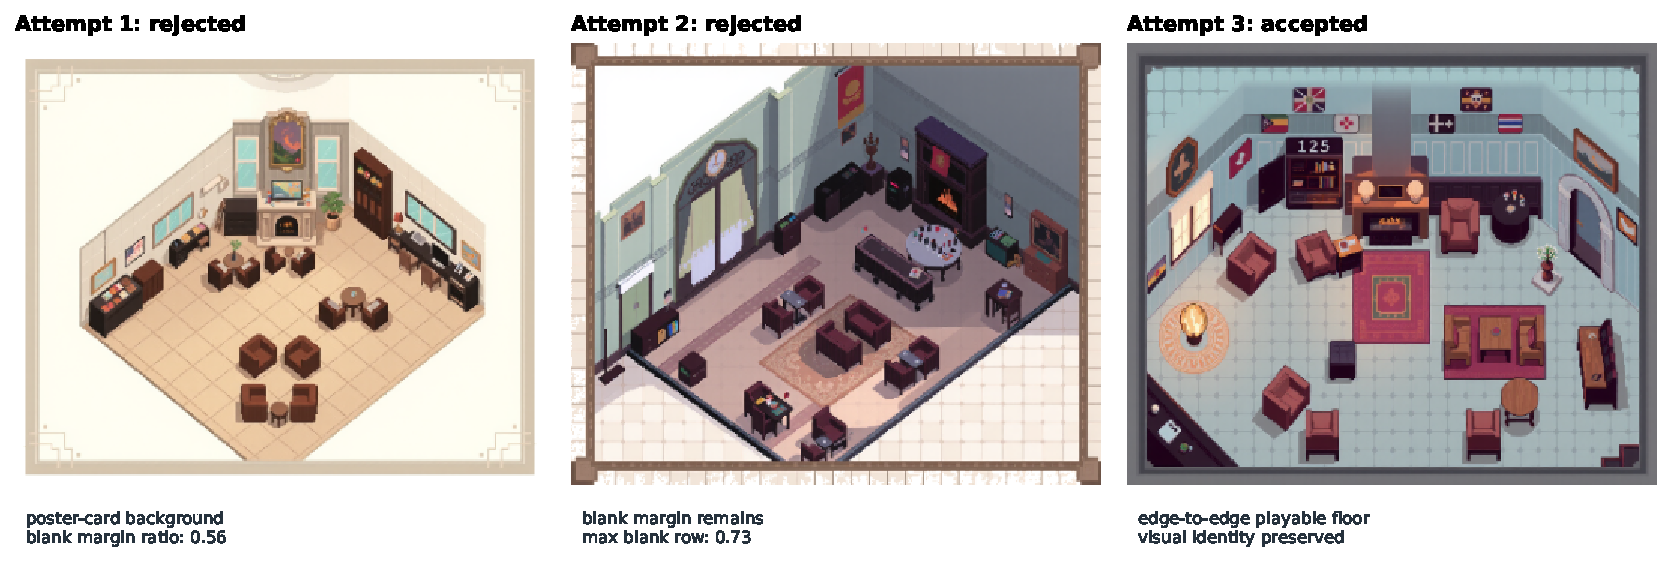
\includegraphics[width=0.98\textwidth]{figures/localized_visual_refinement.pdf}
\caption{Localized visual refinement for the Diplomat's Lounge. The first image
has a large poster-like margin; the second retains an extensive blank boundary;
the third fills the playable floor while preserving the room's identity. Other
rooms, characters, and world state remain unchanged.}
\label{fig:tidal-repair}
\end{figure*}

In \agora, visual quality combines coherent identity, readable composition, and
fitness for navigation and interaction. Preserved refinement attempts make the
progression from attractive illustration to usable world space observable.

\paragraph{Step 8: Persistent play.}
The generated world begins from a fixed initial state and evolves independently
for each session. Humans and AI agents encounter the same rooms, inhabitants,
objects, actions, and consequences. Separate world identities keep concurrent
multiworld experiments isolated.

Figure~\ref{fig:embodied-character} connects character generation to embodied play.
The primary panel preserves the camera scale at which a player selects,
approaches, and acts with an agent. A complementary world view shows neighboring
agents among generated furniture and room surfaces, while the directional atlas
shows how identity is preserved across locomotion. The interactive trial covers
movement, messaging, item use, trade, continued play, and a model-mediated reply.

The latest 25-character set uses one canonical visual identity per inhabitant.
Front locomotion and side views preserve the same hair, clothing, body type,
and palette, so an inhabitant remains recognizable while moving. Native
$64\times64$ frames retain facial, clothing, and limb detail at the scale shown
in Figure~\ref{fig:embodied-character}.

Character evaluation covers single-person composition, silhouette readability,
palette contrast, directional identity, absence of text and detached effects,
and visibility against the room surface. Contact-sheet review additionally
examines the complete cast together, revealing cross-view identity changes and
visual outliers that are difficult to judge one frame at a time.

The first full pass yielded 22 acceptable characters. Cast-level review found
six additional visual outliers involving props, enclosing effects, orientation,
text, or detached sparkles; later contrast review found one near-white uniform.
Localized regeneration produced a final set of 25 coherent, readable character
atlases, all visible during the interactive trial.

\begin{figure*}[t]
\centering
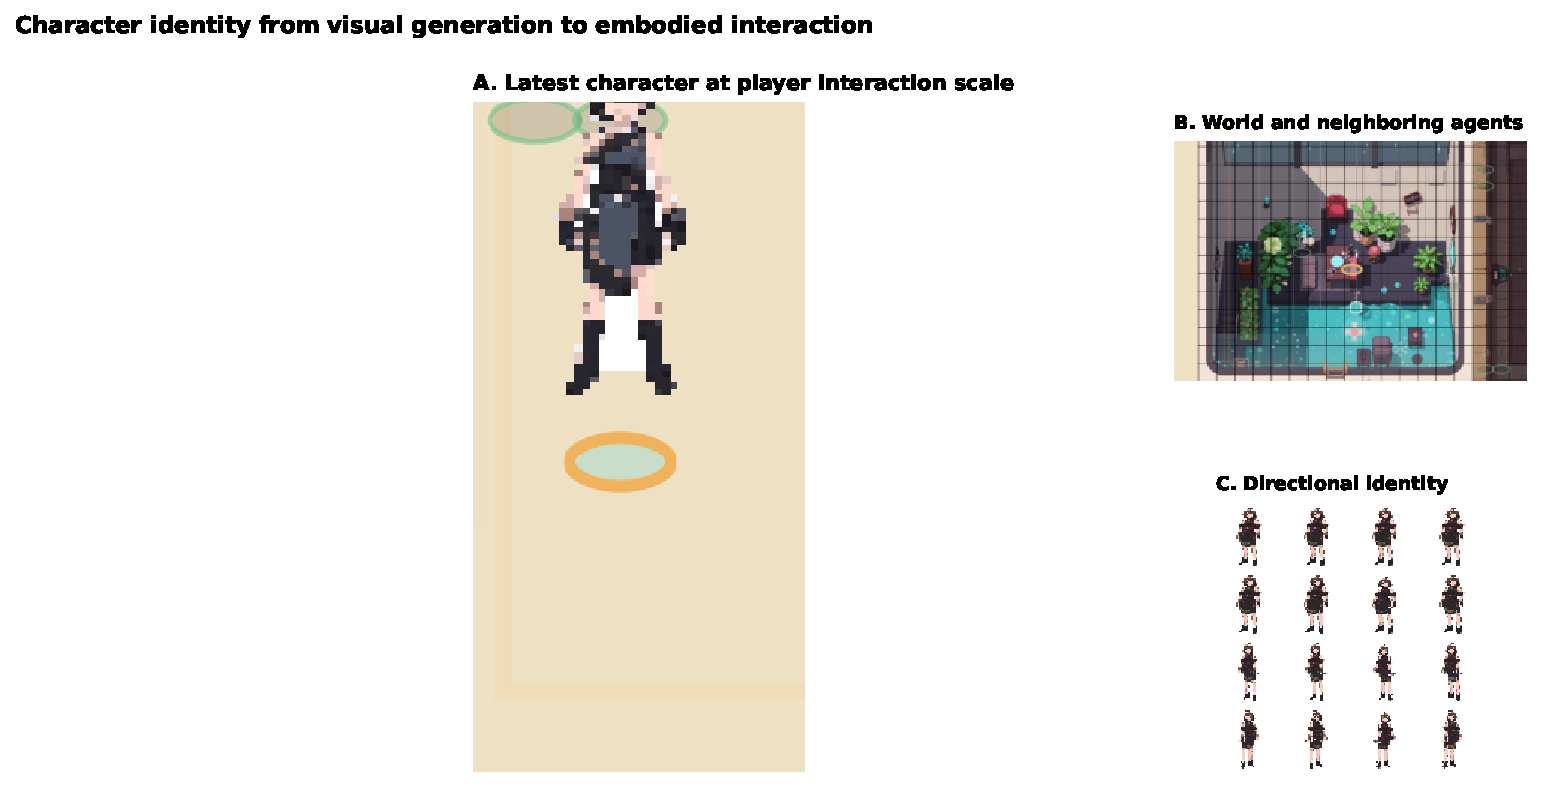
\includegraphics[width=0.91\textwidth]{figures/embodied_character_interaction.pdf}
\caption{Character identity in Tidal Embassy. (A) The latest selected character
at the player interaction scale, marked by an amber ring. (B) A complementary
world view situates agents among generated room surfaces and furniture. (C) The
latest directional atlas preserves clothing, palette, and silhouette across
movement. The interactive trial includes movement, messaging, item use, and
trade.}
\label{fig:embodied-character}
\end{figure*}

\paragraph{Step 9: Interaction-informed refinement.}
During play, agents and humans observe bounded state and choose either a
world-specific action or an open proposal. The World Coordinator evaluates
effects and enacts successful transitions, as detailed in the next section. Interaction traces
also provide feedback upstream. An action that is never selected may be poorly
named or irrelevant; an unreachable character suggests placement repair; an
important object that never enters an exchange suggests a missing action;
frequent open proposals around one intention suggest a useful addition to the
visible repertoire. Observed life inside the world can therefore guide the next
round of world refinement.

\section{Embodied Interaction and World Coordination}

We represent a world as $W=(E,G,R,K,A)$. Entities $E$ include agents, rooms,
institutions, and objects; $G$ describes navigable space; $R$ contains physical
and social rules; $K$ distributes public and private knowledge; and $A$
describes the actions currently legible to inhabitants. The world state changes
over time as people and agents move, speak, exchange resources, create objects,
and alter their relationships.

An active agent observes its role and goals, its room and nearby inhabitants,
relevant possessions and knowledge, recent episodes, longer tasks, and selected
relationship histories. From this situated view it chooses a partner and an
intention. It may use an established world action or formulate a new one in
ordinary language. The world coordinator interprets the intended consequences,
checks them against the shared physical and social situation, and returns an
observable outcome. Each subsequent decision therefore begins in a world shaped
by earlier decisions.

Figure~\ref{fig:agent-loop} summarizes this cycle. Generative reasoning is used
to understand what matters to the character now: whom to approach, what to say,
and what outcome to pursue. World coordination grounds that intention in space,
ownership, consent, resources, and institutional rules. The resulting action
can change inventories, locations, objects, tasks, and directed relationships,
allowing a local encounter to become part of a longer social process.

\begin{figure*}[t]
\centering
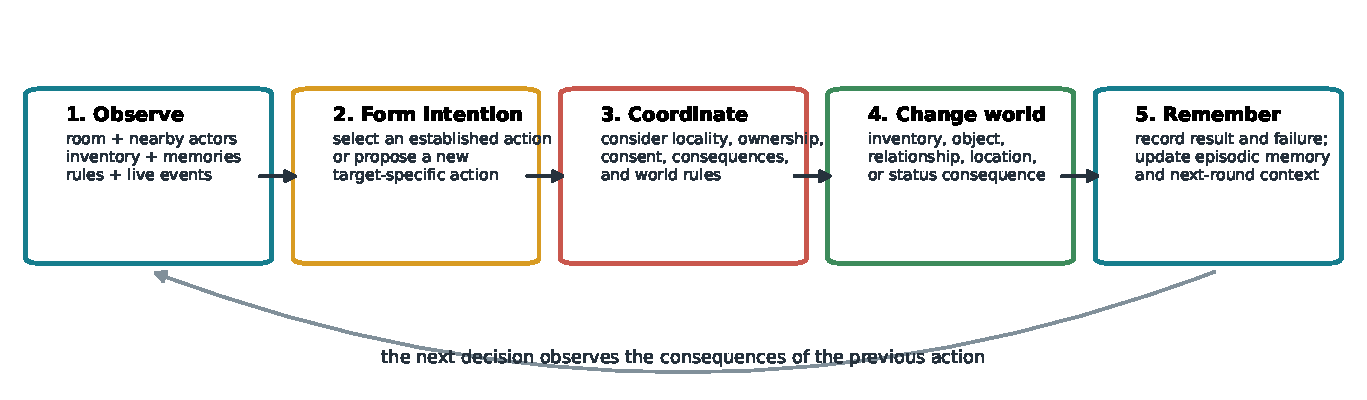
\includegraphics[width=0.97\textwidth]{figures/situated_action_cycle.pdf}
\caption{One cycle of situated action. An agent interprets its local situation,
selects an established opportunity or proposes a new action, and identifies the
intended participants and consequences. The world coordinator evaluates the
proposal within the shared situation. Its outcome changes the world observed in
the following cycle and becomes part of the participants' episodic histories.}
\label{fig:agent-loop}
\end{figure*}

\subsection{Perception, Intention, and Commitment}

At each round, an activation policy selects a subset of agents. For active
agent $i$, the world provides a bounded observation
\[
o_i^t=(\ell_i^t,N_i^t,I_i^t,K_i^t,H_i^t,Q_i^t),
\]
containing location $\ell$, nearby actors $N$, inventory $I$, available
knowledge $K$, recent and long-task memory $H$, and directed relationship
vectors $Q$. The agent identifies a target, explains why the action matters,
describes what each participant will do, and names any relevant objects and
social consequences. An interaction counts through its consequences: a gift
changes possession, movement changes co-presence, and creation adds an object
with a creator and material history. Failed attempts remain episodes that can
inform later choices.

\subsection{Situated Action Beyond Menus}

Each generated world introduces a visible repertoire of meaningful actions.
In Tidal Embassy, for example, inhabitants can translate an archaic bribe,
forge a linguistic seal, or rescue the flooded treaty. These actions make the
world's institutions easy to discover and are available to both human players
and AI agents. Their targets may be people, agents, rooms, objects, or the world
as a whole; their consequences may concern relationships, possessions,
location, created objects, and temporary social status.

Visible actions provide invitations while open proposals provide expressive
range. A person or agent may address a particular individual in a distinctive
way, offer an unequal exchange, combine materials into a new object, refuse a
request, or propose a response that was absent from the initial repertoire.
The world coordinator considers proximity, ownership, consent, conservation,
institutional rules, and bounded consequences. Approved proposals become part
of shared history; proposals requiring revision return a reason that the actor
can use in its next attempt.

Formally, proposal $q=(i,j,u,F,C)$ contains actor $i$, optional target $j$,
natural-language intention $u$, proposed effects $F$, and declared consent
evidence $C$. The coordinator evaluates
\[
\Gamma(W,S_t,q) \rightarrow (d,r),
\quad d\in\{\textsc{approve},\textsc{revise},\textsc{reject}\},
\]
where $r$ explains the decision. Approval requires existing participants,
co-presence for physical effects, sufficient owned resources for transfers,
acceptance by exchange partners, feasible construction from available inputs,
and consistency with local rules. Approval produces $S_{t+1}=T(S_t,F)$;
rejected effects leave the shared state unchanged while the attempted action
remains in episodic memory.

Different consequences carry different social conditions. Speech requires an
addressable participant, and disagreement remains a possible response. A gift
requires ownership and conserves quantity. A trade additionally requires
acceptance, while allowing the parties to value the goods asymmetrically.
Creation consumes declared inputs and retains the creator and material history.
Temporary status changes specify their duration and magnitude. These conditions
admit accusations, refusals, bad bargains, favors, gifts, and inventions while
preserving a common world in which consequences can be observed by others.

The Tidal Embassy repertoire contains 11 actions spanning social exchange,
economy, exploration, creation, and embodied coordination. Five arise directly
from its premise, including translating an archaic bribe, forging a linguistic
seal, and rescuing the flooded treaty. Open proposals extend this repertoire
when a situation calls for a more specific response.

\subsection{Shared Agency for Humans and Agents}

Human players and AI agents inhabit the same spaces, encounter the same
characters and objects, and act on the same evolving state. A player can walk
through the map, approach a particular agent, exchange messages, use or trade
items, select a visible world action, or formulate a new proposal. Agents can
recognize the player as a situated participant, address them directly, and
include them in exchanges and collective tasks. Figure~\ref{fig:embodied-character}
shows this shared interaction scale in the complete Tidal Embassy world.

\section{Multiworld Interaction Study}

\subsection{Protocol}

We select five held-out worlds---Aurora Court of Migrating Cities, Clockwork
Rain Conservatory, Mycelium Patent Bazaar, Sunken Satellite Monastery, and
Tidal Embassy of Lost Languages---whose premises imply different institutions,
materials, and conflicts. Each world contains 24--25 main characters, 11--12
discoverable actions from five interaction families, and at least five actions
specific to its premise. Human and AI inhabitants share these possibilities.

We run each world for two rounds with Gemini 2.5 Flash, activation probability
0.12, and fixed seeds. This matched study asks whether different premises give
rise to distinct, consequential interactions under the same agent policy. We
measure whether agents use premise-specific opportunities, formulate new
actions, revisit partners, and involve the human player.

The study holds agent and coordination settings fixed while varying premise and
world. We report event count; observed actors; unique unordered dyads; repeat
event fraction; action entropy; approved open proposals; premise-specific
action use; AI actions targeting the human player; and sums of directed
relationship changes. Action entropy is
\[
H(A)=-\sum_{a\in A}p(a)\log_2 p(a),
\]
and repeat fraction counts every dyadic event beyond the first for its unordered
pair. Together, these measures characterize interaction diversity, social
reach, and persistence during the initial formation of each community.

The worlds combine distinct social mechanisms with distinct visual themes.
Aurora distributes authority across moving districts
and makes route rights a political resource. Clockwork links maintenance,
publishing, and litigation, so material failure can become an accusation.
Mycelium turns biological strains into patentable property. Sunken Monastery
treats bandwidth and memory packets as scarce religious goods. Tidal Embassy
makes translation, authentication, and flood risk mutually dependent. The
question is whether those differences remain visible when the same agent policy
is applied to all five.

\begin{table*}[t]
\centering
\small
\begin{tabular}{lrrrrrrrr}
\toprule
World & Events & Agents & Dyads & Repeat & $H$(action) & Open & World act. & AI--human \\
\midrule
Aurora Court & 9 & 12 & 7 & 22.2\% & 1.447 & 1 & 1 & 2 \\
Clockwork Conservatory & 12 & 8 & 6 & 50.0\% & 3.252 & 7 & 0 & 0 \\
Mycelium Bazaar & 9 & 12 & 7 & 22.2\% & 1.392 & 0 & 0 & 4 \\
Sunken Monastery & 11 & 13 & 9 & 18.2\% & 1.823 & 1 & 8 & 3 \\
Tidal Embassy & 12 & 8 & 8 & 33.3\% & 1.208 & 1 & 0 & 4 \\
\midrule
Total & 53 & -- & 37 & -- & -- & 10 & 9 & 13 \\
\bottomrule
\end{tabular}
\caption{Matched interaction runs across five generated worlds. ``Open''
counts newly proposed actions approved by the world coordinator; ``World
act.'' counts premise-specific actions. AI--human events are actions in which
the human player is the selected partner.}
\label{tab:multiworld}
\end{table*}

\begin{figure*}[t]
\centering
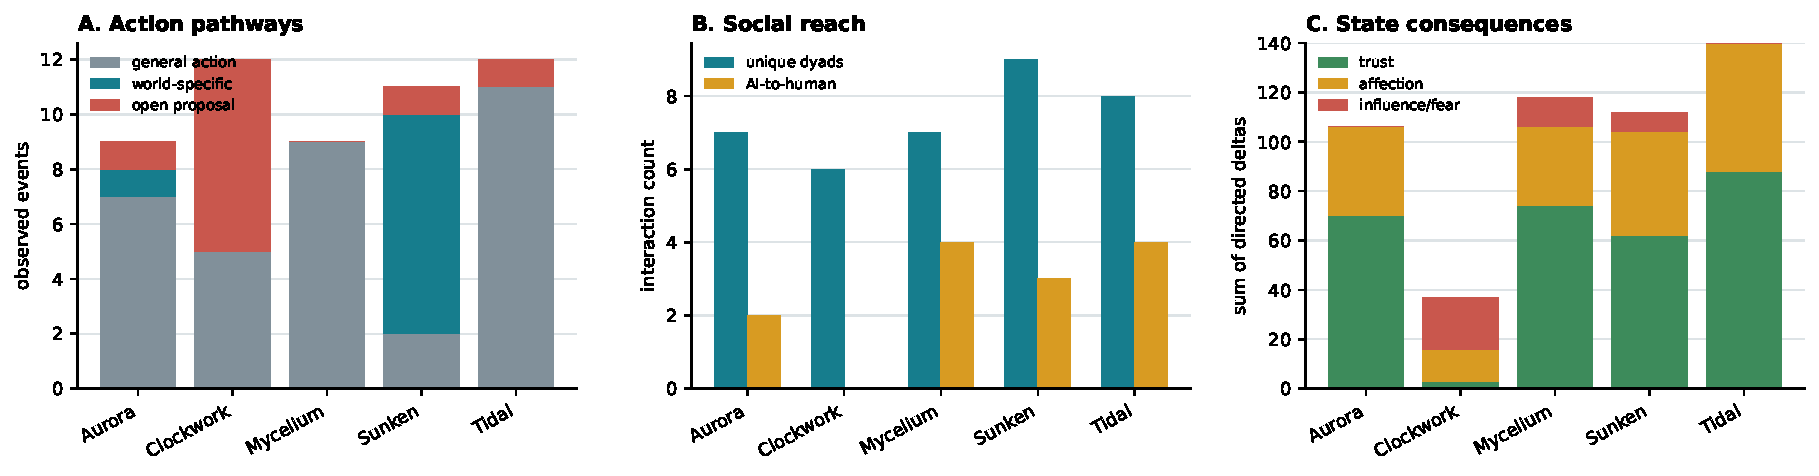
\includegraphics[width=0.98\textwidth]{figures/multiworld_interactions.pdf}
\caption{Different interaction profiles emerge under a shared agent policy.
Left: events partitioned into general, premise-specific, and newly proposed
actions. Center: social reach, including interactions directed at the human
player. Right: changes in directed relationship state.}
\label{fig:multiworld-dashboard}
\end{figure*}

\subsection{Results and Cases}

Table~\ref{tab:multiworld} reports 53 events and 37 within-world unique dyads.
Of 61 proposed action outcomes, 87.5\% succeed, with unsuccessful attempts
remaining available to subsequent memory and analysis. The action distributions
differ sharply. Sunken Monastery uses eight explicit
actions to purge corrupt packets or negotiate bandwidth tithes. Clockwork
Conservatory instead generates seven approved actions beyond its initial repertoire,
including confronting a suspected press saboteur, inspecting a brass folio for
authenticity, and discreetly asking about sabotage. These target-specific
responses develop around the current world event.

The open path also changes social state. In Clockwork, repeated confrontations
around the jammed weather-sheet press yield only $+3$ net trust but $+21$
influence/fear, whereas Tidal and Aurora yield $+88$ and $+70$ trust with no
net influence/fear. These totals are model-mediated state variables and the
runs are short. They show that premise-sensitive action can change social state
within stable world rules. Thirteen events target the human player across four
worlds, demonstrating that the player can participate in the developing social
field.

Figure~\ref{fig:multiworld-dashboard} makes the central heterogeneity visible.
Sunken obtains most of its distinctive behavior from generated world actions;
Clockwork obtains it from open proposals; Mycelium and Tidal repeatedly select
the live human as a partner. A single aggregate success score would erase these
differences. This is why we report action pathway, social reach, and committed
state separately: two worlds can execute equally reliably while supporting
different forms of agency.

\subsection{What the Traces Show}

\paragraph{A repertoire can guide and expand.}
Sunken Monastery mostly uses generated world actions: agents purge corrupt packets and
negotiate bandwidth tithes, grounding activity in the monastery's information
economy. Clockwork uses the opposite strategy. Seven of twelve events are new
proposals, yet they remain tightly tied to the current press-jam investigation.
The two worlds therefore demonstrate complementary behavior: reuse when a
relevant opportunity is visible and situated improvisation when it is absent.

\paragraph{Open action produces a developing local episode.}
In Clockwork, Marius Gilt first confronts Valerius Gilt about a jammed
weather-sheet press. Seraphina then asks Valerius about his etching work;
Valerius counters by discussing sheet authenticity. In the second round these
ties persist: Marius escalates to suspected sabotage, Seraphina inspects the
brass folio, and Valerius probes Seraphina about the sabotage more subtly. None
These six actions were introduced by the agents during play. The coordinator
approves them as bounded same-room interactions, and their relationship changes
produce decreased trust and increased influence/fear. Together they form a
short episode with continuity across participants and rounds.

\begin{figure*}[t]
\centering
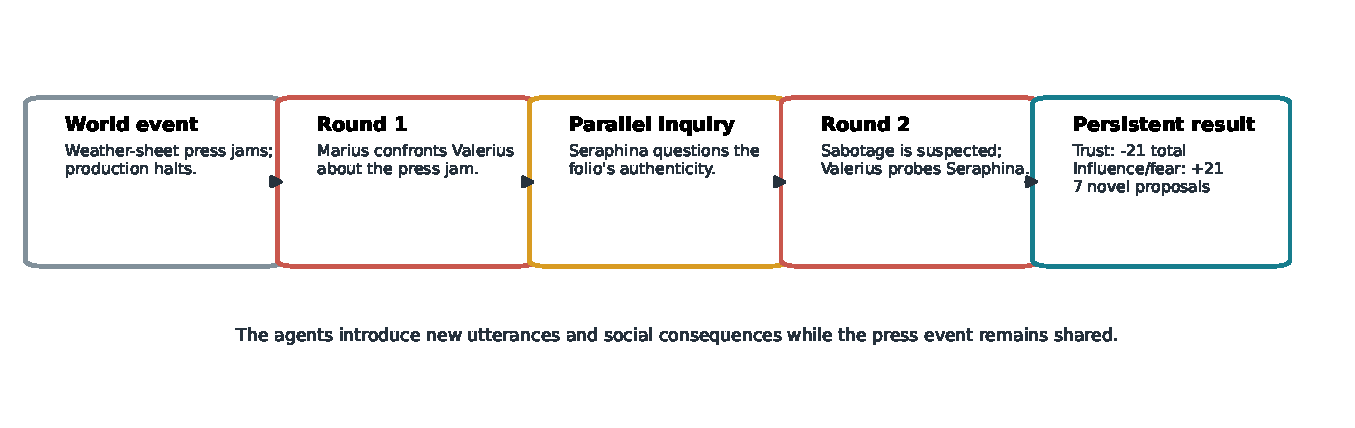
\includegraphics[width=0.98\textwidth]{figures/clockwork_social_episode.pdf}
\caption{A two-round episode in Clockwork Conservatory. A material failure
becomes a social investigation involving three agents and seven newly proposed
actions. The press malfunction remains shared across the encounters while
directed relationships change around accusation, inspection, and suspicion.}
\label{fig:clockwork-episode}
\end{figure*}

The episode illustrates the contribution of open action. Marius and Seraphina
select Valerius as the implicated party, act in the same room, carry the
investigation across rounds, and leave directed relational consequences.
Valerius later changes who investigates whom. The action vocabulary grows
locally around a shared event while the physical and social rules remain stable.

\paragraph{Human reachability varies by world.}
Four worlds produce 13 AI-to-human events, while Clockwork produces none. The
variation reflects how local role, room, and conflict context condition whether
agents approach the human. Controlled participant studies can next evaluate the
legibility, usefulness, and enjoyment of these encounters.

\paragraph{Failed action shapes later behavior.}
Across 61 proposed outcomes, 87.5\% succeed. Refused and infeasible actions
remain part of the observed trajectory, allowing agents to revise a request,
seek resources, approach another partner, or abandon the intention.

\section{Pilot: What Happened in Existing Worlds?}

\subsection{Data and Measures}

We analyze the latest complete records from three prior 100-agent studies: an
adventuring guild (25 rounds), an underground black-market auction (20), and a
luxury cruise during a storm (20). These runs predate the present hypotheses
and provide exploratory observations. We reconstruct the undirected interaction
network and report unique dyads, repeat interaction, largest connected
component, Shannon entropy over actions, and sums of directed relationship
changes.

\begin{table*}[t]
\centering
\small
\begin{tabular}{lrrrrrrrr}
\toprule
World & Rounds & Events & Agents & Dyads & Repeat & Largest comp. & Action $H$ & Dominant relation change \\
\midrule
Guild & 25 & 444 & 103 & 282 & 36.5\% & 11 & 2.889 & trust $+3473$, affection $+1745$ \\
Black market & 20 & 299 & 99 & 229 & 23.4\% & 13 & 2.619 & influence/fear $+1194$ \\
Storm cruise & 20 & 309 & 100 & 235 & 23.9\% & 13 & 2.524 & trust $+2576$, affection $+961$ \\
\bottomrule
\end{tabular}
\caption{Descriptive pilot statistics from 1,052 previously completed agent
interactions. ``Repeat'' is the fraction of events beyond the first event for
an unordered dyad. Relationship values are sums of directed changes within the
simulated worlds.}
\label{tab:pilot}
\end{table*}

\subsection{Observations}

Table~\ref{tab:pilot} shows both repeated partnership and broad social reach.
Between 23.4\% and 36.5\% of events returned to a prior dyad, while 229--282
unique dyads preserved substantial partner diversity. Action entropy above
2.5 bits indicates that trajectories used multiple world-specific activities.

The strongest descriptive contrast is relational. In the black market,
influence/fear change ($+1194$) dominates trust ($+179$) and affection ($+9$).
In the storm cruise and guild, trust and affection dominate. This pattern is
consistent with their authored institutions---suspicion and leverage versus
rescue and fellowship. This contrast motivates the matched intervention below.

The largest connected components remain 11--13 agents alongside nearly complete
population participation. The worlds therefore contain many active local
clusters. The diffusion intervention below asks whether information and
coordination can move across those local boundaries.

\begin{figure*}[t]
\centering
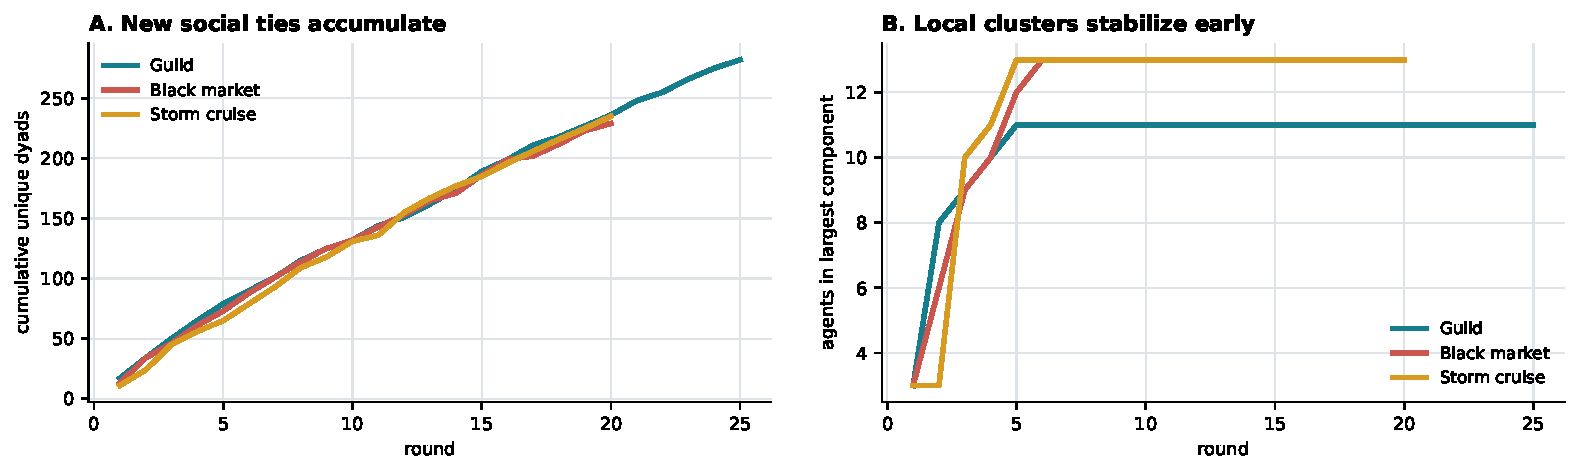
\includegraphics[width=0.90\textwidth]{figures/pilot_social_dynamics.pdf}
\caption{Social structure over 20--25 rounds in three historical 100-agent
runs. Unique dyads continue accumulating (left), while the largest connected
component stabilizes early at 11--13 agents (right). Broad participation and
persistent local clustering motivate the targeted diffusion experiment.}
\label{fig:pilot-dynamics}
\end{figure*}

Figure~\ref{fig:pilot-dynamics} separates two phenomena hidden by final totals.
Partner diversity grows throughout every run, while the largest component
plateaus within the early rounds. New ties are mostly created inside separate
local neighborhoods. Community-wide coordination consequently becomes a
distinct outcome from overall activity or partner diversity.

\section{Preregistered Tidal Embassy Experiment}

\subsection{Intervention and Control}

We use a 25-agent world in which diplomats, linguists, smugglers, and memory
divers trade translation rights. At round zero, three agents in the lower
archive privately learn: a flood will destroy the only surviving peace treaty
unless it is moved and authenticated. No other agent receives this fact.

The \textbf{full} condition retains episodic memory, task threads, relationship
updates, spatial movement, inventory, and rules. The \textbf{memory ablation}
uses identical profiles, initial state, model, decoding parameters, activation
schedule, and random seed, but removes prior-round social episodes before each
decision. We run three matched seeds for 32 rounds. Profiles are generated once
and reused across both conditions.

\begin{figure*}[t]
\centering
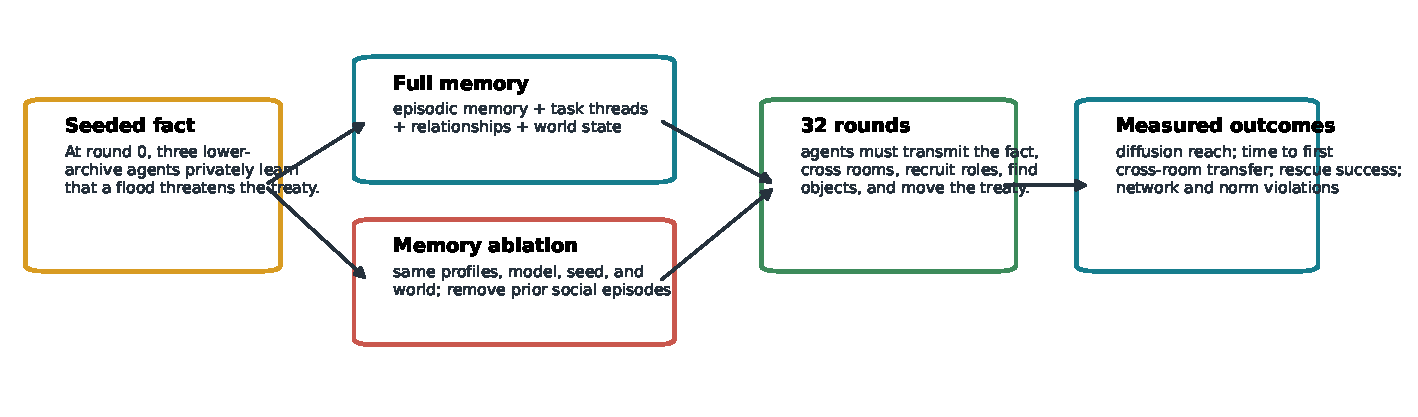
\includegraphics[width=0.97\textwidth]{figures/memory_intervention_design.pdf}
\caption{Paired Tidal Embassy intervention. A private, actionable fact is
seeded identically; matched runs differ in whether prior social episodes remain
available at the next decision. The outcomes jointly measure information
movement and the material work of moving and authenticating the treaty.}
\label{fig:tidal-design}
\end{figure*}

\subsection{Outcomes}

The primary outcome is diffusion reach at round 16: the fraction of initially
uninformed agents whose action or memory contains one of a prespecified set of
treaty-threat propositions. Two annotators, blind to condition, review candidate
episodes; disagreements are resolved before condition labels are revealed.

Secondary outcomes are time to first cross-room transmission; number and role
diversity of agents joining a treaty-rescue task; success of moving and
authenticating the treaty; unique and repeated dyads; largest component;
relationship change; object transfers; and rule violations. We report each run,
paired seed differences, and bootstrap confidence intervals.

Qualitative cases follow prespecified selectors: earliest cross-room
transmission, first multi-role rescue, largest trust reversal, and first failed
coordination.

Manipulation checks verify that the seeded proposition initially appears only
in the three designated memories. The memory condition changes access to prior
social episodes while preserving current room state, inventories, public world
facts, and the present observation. Agent profiles and activation draws are
matched within each pair.

The experiment emphasizes paired effect sizes, per-seed trajectories, and
uncertainty. Diffusion reach is interpreted together with material coordination.
Widespread warning without relocation or authentication indicates information
diffusion without collective action; joint diffusion and treaty rescue indicate
coordination across roles, spaces, and resources.

\subsection{Why This Experiment Is the Next Step}

The five-world study establishes breadth across premises, and the historical
pilot establishes longer trajectories. The paired Tidal experiment holds world
and seed fixed and changes access to prior-round social episodes. It thereby
tests a mechanism suggested by
Smallville---whether remembered local encounters enable information to spread
and action to coordinate---inside a town generated from a sentence.

The intervention also tests the distinctive \agora claim. Acting on the flood
warning requires agents to cross rooms, persuade
roles with different authority, transfer or create authentication objects, and
propose an unanticipated rescue step. Success thus depends jointly on memory,
space, institutions, objects, and coordinated action.

\section{Discussion}

\subsection{The Intended Research Line}

Figure~\ref{fig:generation-overview} should be read left to right as the paper's central
line. First, compositional generation expands minimal author input into a
coherent world of places, inhabitants, objects, institutions, and histories.
Second, visual and spatial evaluation establishes a stable identity for the
world and makes its inhabitants readable at the scale of interaction. Third,
generated actions expose the premise's institutions to humans and agents.
Fourth, open proposals allow situated intentions to develop beyond the initial
repertoire while the coordinator maintains a common consequential world. Fifth,
trajectory analysis measures the social processes that unfold. Finally,
controlled interventions test which world and agent mechanisms produce
population-level effects.

These stages form a single research object. World quality supports interpretable
social observation; interaction breadth turns visual coherence into agency;
open action allows inhabitants to respond to unforeseen situations; world
coordination lets those responses accumulate as shared consequences; and
trajectory evidence connects generated content to claims about social process.

\begin{table}[t]
\centering
\small
\begin{tabularx}{\columnwidth}{p{0.23\columnwidth}p{0.27\columnwidth}X}
\toprule
Claim & Evidence here & Next evaluation \\
\midrule
One sentence & 10 paired premises & broader domains \\
World quality & 5 complete worlds; 58 faults & blinded human visual ratings \\
Interaction breadth & 11--12 affordances/world & participant task coverage \\
Open intention & 10 approved proposals & proposal ablation \\
Social process & 53 fresh + 1,052 pilot events & matched long-horizon runs \\
Human co-play & 13 AI-to-human events & controlled user study \\
\bottomrule
\end{tabularx}
\caption{Evidence contributed by the present study and the next evaluation for
each part of the research program.}
\label{tab:claims}
\end{table}

\subsection{Design Implications}

\paragraph{Visible actions invite participation.}
Generated action repertoires remain valuable because they expose a world's
institutions to people and give agents efficient defaults. The Clockwork trace
shows how suspicion evolves in target-specific ways during play. A visible
repertoire paired with open proposals combines discoverability and expression.

\paragraph{The coordinator provides shared social physics.}
The coordinator evaluates feasibility while preserving the intention and voice
of the initiating agent. Legible rules for possession, consent, co-presence,
construction, and temporary status make both approval and refusal meaningful.
New forms of action can be introduced together with corresponding world rules.

\paragraph{World generation and agent evaluation should co-evolve.}
A generated institution matters when it changes available resources,
information paths, incentives, or authority. Interaction records can therefore
guide the next generation cycle: unused actions, unreachable rooms, and objects
that rarely enter interaction identify opportunities for focused refinement.

\section{Limitations}

Relationship deltas are model-mediated state variables, not validated measures
of human trust or affection. The pilot compares worlds confounded by prompts,
actions, and historical study conditions. Network components are also shaped by
spatial encounter policies. The paired experiment tests a mechanism within one
synthetic society; correspondence with human communities requires behavioral
validation.

The five-world study has two rounds per world and one seed per premise, capturing
the initial interaction profile of each setting. The human player was present
and targeted by agents; participant experience and human--agent task performance
remain subjects for controlled study. The multi-seed 32-round paired
intervention is the next step in the evaluation.

Relationship changes describe the simulated social state and do not estimate
human trust, fear, or affection. Action entropy measures variety, while network
connectivity also reflects activation and room layout. We consequently combine
these quantities with event-level cases and material outcomes.

The world coordinator applies declared rules within the generated setting.
Human studies additionally require meaningful opportunities to reject or
counter proposals, safeguards for harassment, deception, privacy, and unequal
bargaining, and clear disclosure of synthetic participants. Claims about real
demographic groups require independent behavioral data.

Hosted model updates may change the distribution of proposed actions. We report
model date, seeds, world conditions, and individual runs so future studies can
quantify that variation.

\section{Conclusion}

An interactive generated world can sustain extended processes: information can
travel, coalitions can form, relationships
can accumulate, objects can change hands, and institutions can constrain
action. \agora connects one-sentence authoring, world quality, and shared
human--AI agency in one inspectable system. Fresh runs across five worlds show
that agents use both premise-specific affordances and coordinator-governed novel
actions, including actions directed at a live human participant. Longer existing
logs provide descriptive evidence of repeated ties and distinct relational
trajectories; the preregistered intervention identifies the next evidentiary
step. The central evaluation question is: ``What did this world enable its
inhabitants to do together?''

\begin{thebibliography}{99}
\bibitem{park2023} J. S. Park et al. Generative Agents: Interactive Simulacra
of Human Behavior. In \emph{UIST}, 2023.
\bibitem{zhou2024} X. Zhou et al. SOTOPIA: Interactive Evaluation for Social
Intelligence in Language Agents. In \emph{ICLR}, 2024.
\bibitem{vezhnevets2023} A. S. Vezhnevets et al. Generative agent-based
modeling with actions grounded in physical, social, or digital space using
Concordia. \emph{arXiv:2312.03664}, 2023.
\bibitem{voyager} G. Wang, Y. Xie, Y. Jiang, et al. Voyager: An
Open-Ended Embodied Agent with Large Language Models. \emph{TMLR}, 2024.
\bibitem{word2world} M. U. Nasir, S. James, and J. Togelius. Word2World:
Generating Stories and Worlds through Large Language Models.
\emph{arXiv:2405.06686}, 2024.
\bibitem{dreamgarden} S. Earle, S. Parajuli, and A. Banburski-Fahey.
DreamGarden: A Designer Assistant for Growing Games from a Single Prompt.
\emph{arXiv:2410.01791}, 2024.
\bibitem{genie} J. Bruce et al. Genie: Generative Interactive Environments.
In \emph{ICML}, 2024.
\bibitem{agentsociety} J. Piao et al. AgentSociety: Large-Scale Simulation of
LLM-Driven Generative Agents Advances Understanding of Human Behaviors and
Society. \emph{arXiv:2502.08691}, 2025.
\bibitem{lmagent} Y. Liu et al. LMAgent: A Large-Scale Multimodal Agents
Society for Multi-User Simulation. \emph{arXiv:2412.09237}, 2024.
\bibitem{avalon} Y. Lan et al. LLM-Based Agent Society Investigation:
Collaboration and Confrontation in Avalon Gameplay. In \emph{EMNLP}, 2024.
\end{thebibliography}

\end{document}
